\documentclass[../main.tex]{subfiles}
\begin{document}

\begin{question}
    Find all of the Nash equilibria and subgame perfect Nash equilibria of the following game.

    \centering
    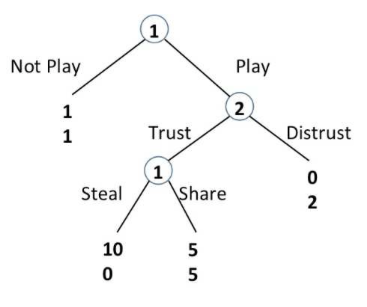
\includegraphics[width=0.4\textwidth]{Question3-1.png}
	%TODO: tikzify for more awesomeness
\end{question}

\begin{solution} 
Let's start by creating the induced normal form matrix of this game. 
There are two decision nodes for player one so to find all the pure strategies we have to use the cartesian product of the options in the two nodes. This results in the four rows.
Because there is only one decision node for player 2 only two columns are needed.
Below is the corresponding matrix with the best responses marked ($\underline{underline}$ for row player, $\overline{overline}$ for column player): 
\begin{center}
	\setlength\extrarowheight{1pt} %extra row height for overline
	\begin{tabular}{|l|c|c|}
		\hline
		& $Trust$ & $Distrust$ \\
		\hline
		$(Not Play,Steal)$ & $(1,\overline{1})$ & \textcolor{blue}{$\mathbf{(\underline{1},\overline{1})}$} \\
		\hline
		$(Not Play,Share)$ & $(1,\overline{1})$ & \textcolor{blue}{$(\underline{1},\overline{1})$} \\
		\hline
		$(Play,Steal)$ & $(\underline{10},0)$ & $(0,\overline{2})$ \\
		\hline
		$(Play,Share)$ & $(5,\overline{5})$ & $(0,2)$ \\
		\hline
	\end{tabular}
\end{center}
\begin{itemize}
	\item General Nash equilibria consist of best responses for both players. So if a payoff vector has been both underlined for player one and overlined for player two it's an Nash Equilibrium. This gives us the following \textcolor{blue}{Nash equilibria}: 
	$$\{\Big((Not Play, Steal),Distrust)\Big),\Big((Not Play, Share),(Distrust)\Big)\}$$
	\item Next we have to look at Subgame Perfect NEs (SPNEs).
		If a profile is a SPNE it is also a Nash Equilibrium ($P \in SPNE \rightarrow P \in NE$).
		Because of this, non-Nash Equilibria profiles can never be SPNE ($P \notin NE \rightarrow P \notin SPNE$). Thanks to this property we can only consider the NEs we found and check whether any of them are also SPNEs.
		Let us now look at the two NEs we found.

		\textcolor{blue}{$\mathbf{\Big((Not Play, Steal),Distrust)\Big)}$}:\\
		If we consider the second node of player one as subgame we see that $Steal$ is the best option here so there is no profitable deviation from restriction $Steal$ for this subgame ($10>5$).
		Next we consider the decision node of player two and below as a subgame.
		Again none of the players can deviate to increase their profit.
		If player two choses $Trust$ (instead of restriction $Distrust$) it will result in a zero payoff which is lower than the payoff received under the restriction ($0<2$).
		We already considered the options of player one in the left branch of this subgame and found no profitable deviations there.
		The last subgame is the whole game and we already know the outcome here.
		Because we found no profitable deviation in any of the subgames, this profile is a \textbf{Subgame Perfect Nash Equilibrium}.

		\textcolor{blue}{$\Big((Not Play, Share),Distrust)\Big)$}:\\
		If we consider the second node of player one as subgame we see that $Steal$ (instead of restriction $Share$) is the best option here for player one ($10>5$).
		This means there \emph{is} a profitable deviation in some subgame so this strategy profile can NOT be a Subgame Perfect Nash Equilibrium. 
		No further analysis is necessary because one counter example is sufficient.
\end{itemize}
\end{solution}

\begin{question}
In a game where player $i$ has $N$ information sets indexed $n = 1, ..., N$ and $M_n$ possible actions at information set $n$, how many pure strategies does player $i$ have?
\end{question}

\begin{solution}
	From the definition of pure strategies for imperfect information games \egtcite{52} we know that a pure strategie is composed of the $N$ choices made at each information set.
	Since information set $n$ has $M_n$ options we have to multiply all options by eachother to find the amount of all possible pure strategies.
	This gives us
$$\prod\limits_{n=1}^N M_n$$
as solution. 
\end{solution}

\begin{question}[Rain]
Players 1 and 2 must decide whether or not to carry an umbrella when leaving home. They know that there is a 50-50 chance of rain. Each player's payoff is -5 if she does not carry an umbrella and it rains, -2 if she carries an umbrella and it rains, -1 if she carries an umbrella and it is sunny and 1 if she doesn't carry an umbrella and it is sunny. Player 1 learns the weather before leaving home. Player 2 does not, but she can observe player 1's action before choosing her own
\begin{enumerate}
\item Write down the extensive form of this game as a game tree
\item Write down the induced normal form game.
\end{enumerate}
\end{question}

\begin{solution}
\begin{enumerate}
\item Game tree:
\begin{center}
% macro for entering payoffs
\newcommand\payoff[1]{
  \begin{pmatrix} #1 \end{pmatrix}
}
\tikzset{
  % Two node styles for game trees: solid and hollow
  solid node/.style={circle,draw,inner sep=1.2,fill=black},
  hollow node/.style={circle,draw,inner sep=1.2},
}


\begin{tikzpicture}[font=\footnotesize]
  \tikzset{
    level 1/.style={level distance=15mm,sibling distance=40mm},
    level 2/.style={level distance=15mm,sibling distance=20mm},
    level 3/.style={level distance=15mm,sibling distance=10mm},
  }

  \node[solid node,label=above:{N}]{}
  	child{node(r1)[solid node,label=left:{1}]{}
		child{node(rU)[solid node,label=left:{2}]{}
        		child{node[solid node,label=below:{$\payoff{-2\\-2}$}]{}
					edge from parent[red] node[left]{\textcolor{red}{U}}
        		}
            child{node[solid node,label=below:{$\payoff{-2\\-5}$}]{}
				edge from parent[black] node[right]{\textcolor{red}{NU}}
            }
			edge from parent node[left]{\textcolor{red}{U}}
      	}
      	child{node(rNU)[solid node,label=left:{2}]{}
            child{node[solid node,label=below:{$\payoff{-5\\-2}$}]{}
				edge from parent node[left]{\textcolor{red}{U}}
            }
            child{node[solid node,label=below:{$\payoff{-5\\-5}$}]{}
				edge from parent node[right]{\textcolor{red}{NU}}
            }
			edge from parent[black] node[right]{\textcolor{red}{NU}}
        }
		edge from parent[red] node[left]{Rain (0.5)}
	}
	child{node(s1)[solid node,label=left:{1}]{}
    child{node(sU)[solid node,label=left:{2}]{}
            child{node[solid node,label=below:{$\payoff{-1\\-1}$}]{}
				edge from parent node[left]{\textcolor{blue}{U}}
            }
            child{node[solid node,label=below:{$\payoff{-1\\1}$}]{}
				edge from parent node[right]{\textcolor{blue}{NU}}
            }
			edge from parent[black] node[left]{\textcolor{blue}{U}}
        }
        child{node(sNU)[solid node,label=left:{2}]{}
            child{node[solid node,label=below:{$\payoff{1\\-1}$}]{}
				edge from parent[black] node[left]{\textcolor{blue}{U}}
            }
            child{node[solid node,label=below:{$\payoff{1\\1}$}]{}
				edge from parent[blue] node[right]{\textcolor{blue}{NU}}
            }
			edge from parent node[right]{\textcolor{blue}{NU}}
        }
		edge from parent[blue] node[right]{Sunny (0.5)}
  };

  \draw[bend left=15,-, dashed]  (rU) to node [auto] {} (sU);
  \draw[bend left=15,-, dashed]  (rNU) to node [auto] {} (sNU);
\end{tikzpicture}
\end{center}
Note that only the colored outer branches will ever be played if we assume that both players know the rules of the game and they are both playing rationally.
Player one simply looks at the weather to make her decision and player two can base her decision on the decision of the former.
\item Normal form game:
\begin{center}
	    \begin{tabular}{|l|c|c|c|c|}
	    \hline
		& $\textcolor{blue}{U_1}\textcolor{red}{U}$ 		& $\textcolor{blue}{U_1}\textcolor{red}{NU}$ 		& $\textcolor{blue}{NU_1}\textcolor{red}{U}$ 		& $\textcolor{blue}{NU_1}\textcolor{red}{NU}$ 	\\
	    \hline
		$\textcolor{blue}{U_2}\textcolor{red}{U}$ 	  & (-1.5, -1.5) 	& (-3, -1.5)	  & (-1.5, -0.5) 	& \textbf{(-1.5, -2)}		\\
	    \hline
		$\textcolor{blue}{U_2}\textcolor{red}{NU}$  	& (-3, -1.5) 		& (-3, -3)		  & (-3, -0.5) 		& (-3, -2)			\\
	    \hline
		$\textcolor{blue}{NU_2}\textcolor{red}{U}$  	& (-0.5, -1.5) 	& (-3, -0.5) 	  & (-0.5, -0.5) 	& -(0.5, -2)    \\
	    \hline
		$\textcolor{blue}{NU_2}\textcolor{red}{NU}$  	& (-2, -1.5)	 	& (-2, -3) 		 & (-2, -0.5) 		& (-2, -2)		  \\
	    \hline
	    \end{tabular}
    \end{center}
    Note: $NU_i U $ is when player $i$ chooses No Umbrella when it does not rain and chooses Umbrella when it rains.
	The (expected) payoffs shown in the induced normal form game are calculated analogously to the example calculation of the \textbf{top right payoff} below:
	\[
		\begin{pmatrix}U_2U\\NU_1NU\end{pmatrix} = \overbracket{0.5}^{\textcolor{red}{P(rain)}} \underbrace{\begin{pmatrix}-2\\-5\end{pmatrix}}_{\textcolor{red}{(U,NU)}} + \overbracket{0.5}^{\textcolor{blue}{P(sun)}} \underbrace{\begin{pmatrix}-1\\1\end{pmatrix}}_{\textcolor{blue}{(U,NU)}} = \begin{pmatrix}-1.5 \\ -2 \end{pmatrix} = \textbf{\text{(-1.5, -2)}}^T
	\]
\end{enumerate}
\end{solution}

\begin{question}[Investing smartly]
Two players each invest \euro10 in a single long-term project that is executed in two phases. After each phase, the players have to simultaneously decide whether to withdraw their money from the project or not. If one or both of the investors pulls out after the first phase, the project has to shut down prematurely and only \euro12 can be recovered. After phase two, the project yields \euro30. After each phase, if both players withdraw, the money is divided evenly. If only a single player withdraws, she gets back her entire investment and, if applicable, all of the profits (the profit is \euro0 after round 1 and \euro10 after round 2). If none of the player withdraws their money after the second phase, they both receive \euro10.
\begin{enumerate}
\item Write down the extensive form game of this problem as a game tree.
\item Identify all Nash equilibria.
\item Identify all subgame perfect Nash equilibria.
\end{enumerate}
\end{question}

\begin{solution}
\begin{enumerate}
\item Game tree:
\begin{center}

\tikzset{
  % Two node styles for game trees: solid and hollow
  solid node/.style={circle,draw,inner sep=1.2,fill=black},
  hollow node/.style={circle,draw,inner sep=1.2},
}

% macro for entering payoffs
\newcommand\payoff[1]{
  $\begin{pmatrix} #1 \end{pmatrix}$
}
\begin{tikzpicture}[font=\footnotesize]
  \tikzset{
    level 1/.style={level distance=15mm,sibling distance=50mm},
    level 2/.style={level distance=15mm,sibling distance=20mm},
    level 3/.style={level distance=15mm,sibling distance=20mm},
    level 4/.style={level distance=15mm,sibling distance=10mm},
    level 5/.style={level distance=15mm,sibling distance=0mm},
  }

  \node[solid node,label=above:{1}]{}
  	child{node(3)[solid node,label=left:{2}]{}
        		child{node[solid node,label=below:{\payoff{6\\6}}]{}
        			edge from parent node[left]{W}
        		}
        		child{node[solid node,label=below:{\payoff{10\\2}}]{}
        			edge from parent node[right]{NW}
        		}
      	edge from parent node[left]{W}
	}
	child{node(4)[solid node,label=right:{2}]{}
            child{node[solid node,label=below:{\payoff{2\\10}}]{}
              edge from parent node[left]{W}
            }
        child{node[solid node,label=left:{1}]{}
        	child{node(1)[solid node,label=left:{2}]{}
            	child{node[solid node,label=below:{\payoff{15\\15}}]{}
              		edge from parent node[left]{W}
            	}
            	child{node[solid node,label=below:{\payoff{20\\10}}]{}
              		edge from parent node[right]{NW}
            	}
            	edge from parent node[left]{W}
            }
            child{node(2)[solid node,label=right:{2}]{}
            	child{node[solid node,label=below:{\payoff{10\\20}}]{}
              		edge from parent node[left]{W}
            	}
            	child{node[solid node,label=below:{\payoff{10\\10}}]{}
              		edge from parent node[right]{NW}
            	}
            	edge from parent node[right]{NW}
            }
          edge from parent node[right]{NW}
        }
        edge from parent node[right]{NW}
  };
   \draw[-, dashed]  (1) to node [auto] {} (2);
   \draw[-, dashed]  (3) to node [auto] {} (4);

\end{tikzpicture}
\end{center}

\item $[(W,*)$ $(W,*)]$      %TODO vraag: is hier (NW,W) (NW,W) ook niet een Nash equilibrium?
\item $[(NW,W)$ $(NW,W)]$\\ 
	$[( ,W)$ $( ,W)]$

\end{enumerate}
\end{solution}

\begin{question}[Piracy]
In this exercise, we explore what would happen if pirates (ahrrrr) were not only treacherous, selfish and
thirsty for blood, but also extremely intelligent.
Five pirates have obtained 100 gold coins and have to divide up the loot. The captain proposes a distribution of the loot. All pirates then vote on the proposal, and if half the crew or more go “Aye”, the loot is divided as proposed. If the captain fails to obtain support of at least half his crew (including himself), all pirates turn against him and make him walk the plank. The pirates then start over again with the next most senior pirate as captain. Obviously, each pirate prefers any outcome where he survives over any outcome where he dies. Given survival, each pirate wants to maximize the number of gold coins he receives. Given equal amounts of gold, each pirate prefers to throw as many pirates overboard as possible.
Let five pirates be $A,B, C, D$ and $E$ and assume a strict order of seniority where $A$ is more senior than $B$, $B$ is more senior than $C$ and so on. What are the subgame-perfect equilibria of this game?
\end{question}

\begin{solution}
$A > B > C > D > E$
\begin{itemize}
	\item $E$: (100)
	\item $D$: (100, 0)
	\item $C$: (99, 0, 1)
	\item $B$: (99, 0, 1, 0)
	\item $A$: (98, 0, 1, 0, 1)
\end{itemize}
\end{solution}

\begin{question}
\end{question}

\begin{solution}
\end{solution}

\begin{question}
\end{question}

\begin{solution}
\end{solution}

\begin{question}
\end{question}

\begin{solution}
\end{solution}

\begin{question}
\end{question}

\begin{solution}
\end{solution}

\begin{question}
\end{question}

\begin{solution}
\end{solution}

\begin{question}
\end{question}

\begin{solution}
\end{solution}

\end{document}

